\documentclass[a4paper, 11pt]{article}
\usepackage[utf8]{inputenc} 
\usepackage[T1]{fontenc}
\usepackage{lmodern}
\usepackage{graphicx}
\usepackage{hyperref}

\usepackage[french]{babel}

\usepackage{xcolor}
\usepackage{listings}




% Source Code
%\usepackage{color}
%\usepackage{textcomp}
%\usepackage{listings}
%\usepackage{ulem}
%\usepackage[T1]{fontenc}
%\usepackage{times}
% \usepackage{needspace}
 

% Source Code
\usepackage{color}
\usepackage{textcomp}
\usepackage{listings}

\definecolor{source}{gray}{0.85}% my comment style
\newcommand{\myCommentStyle}[1]{{\footnotesize\sffamily\color{gray!100!white} #1}}
%\newcommand{\myCommentStyle}[1]{{\footnotesize\sffamily\color{black!100!white} #1}}

% my string style
\newcommand{\myStringStyle}[1]{{\footnotesize\sffamily\color{violet!100!black} #1}}
%\newcommand{\myStringStyle}[1]{{\footnotesize\sffamily\color{black!100!black} #1}}

% my symbol style
\newcommand{\mySymbolStyle}[1]{{\footnotesize\sffamily\color{violet!100!black} #1}}
%\newcommand{\mySymbolStyle}[1]{{\footnotesize\sffamily\color{black!100!black} #1}}

% my keyword style
\newcommand{\myKeywordStyle}[1]{{\footnotesize\sffamily\color{green!70!black} #1}}
%\newcommand{\myKeywordStyle}[1]{{\footnotesize\sffamily\color{black!70!black} #1}}

% my global style
\newcommand{\myGlobalStyle}[1]{{\footnotesize\sffamily\color{blue!100!black} #1}}
%\newcommand{\myGlobalStyle}[1]{{\footnotesize\sffamily\color{black!100!black} #1}}

% my number style
\newcommand{\myNumberStyle}[1]{{\footnotesize\sffamily\color{brown!100!black} #1}}
%\newcommand{\myNumberStyle}[1]{{\footnotesize\sffamily\color{black!100!black} #1}}

\lstset{
language={},
% characters
tabsize=3,
escapechar={!},
keepspaces=true,
breaklines=true,
alsoletter={\#},
literate={\$}{{{\$}}}1,
breakautoindent=true,
columns=fullflexible,
showstringspaces=false,
% background
frame=single,
aboveskip=1em, % automatic space before
framerule=0pt,
basicstyle=\footnotesize\sffamily\color{black},
keywordstyle=\myKeywordStyle,% keyword style
commentstyle=\myCommentStyle,% comment style
frame=single,%
backgroundcolor=\color{source},
% numbering
stepnumber=1,
numbersep=10pt,
numberstyle=\tiny,
numberfirstline=true,
% caption
captionpos=b,
% formatting (html)
moredelim=[is][\bfseries]{<b>}{</b>},
moredelim=[is][\textit]{<i>}{</i>},
moredelim=[is][\underbar]{<u>}{</u>},
moredelim=[is][\color{red}\uwave]{<wave>}{</wave>},
moredelim=[is][\color{red}\sout]{<del>}{</del>},
moredelim=[is][\color{blue}\underbar]{<ins>}{</ins>},
% smalltalk stuff
morecomment=[s][\myCommentStyle]{"}{"},
%    morecomment=[s][\myvs]{|}{|},
morestring=[b][\myStringStyle]',
moredelim=[is][]{<sel>}{</sel>},
moredelim=[is][]{<rcv>}{</rcv>},
moredelim=[is][\itshape]{<symb>}{</symb>},
moredelim=[is][\scshape]{<class>}{</class>},
morekeywords={true,false,nil,self,super,thisContext},
identifierstyle=\idstyle,
}

\makeatletter
\newcommand*\idstyle[1]{%
\expandafter\id@style\the\lst@token{#1}\relax%
}
\def\id@style#1#2\relax{%
\ifnum\pdfstrcmp{#1}{\#}=0%
% this is a symbol
\mySymbolStyle{\the\lst@token}%
\else%
\edef\tempa{\uccode`#1}%
\edef\tempb{`#1}%
\ifnum\tempa=\tempb%
% this is a global
\myGlobalStyle{\the\lst@token}%
\else%
\the\lst@token%
\fi%
\fi%
}
\makeatother


%\newcommand{\ct}{\lstinline[backgroundcolor=\color{white}]}
%\newcommand{\needlines}[1]{\Needspace{#1\baselineskip}}
\newcommand{\lct}{\texttt}

\lstnewenvironment{code}{%
    \lstset{%
    % frame=lines,
    frame=single,
    framerule=0pt,
    mathescape=false
    }%
    \noindent%
    \minipage{\linewidth}%
}{%
    \endminipage%
}%


\lstnewenvironment{codeWithLineNumbers}{%
    \lstset{%
    % frame=lines,
    frame=single,
    framerule=0pt,
    mathescape=false,
    numbers=left
    }%
    \noindent%
    \minipage{\linewidth}%
}{%
    \endminipage%
}%



\newenvironment{codeNonSmalltalk}
{\begin{alltt}\sffamily}
{\end{alltt}\normalsize}


 
\begin{document}

\section{Introduction}

Le projet Ironmines a été créé pour répondre offrir une interface de
programmation pour faire évoluer le robot Kobuki. L'objectif est
bien-sur de le faire concourir à la coupe de France de Robotique.

\section{Installation}
\subsection{Pour le développement}
Le programme ironmines peut être installer sur n'importe quel machine
linux compatible avec ROS groovy. On choisira Ubuntu 12.04 pour le
développement. Cette partie expliquera comment installer une version
entière du programme pour le développent. Les étapes sont les
suivantes :
\begin{itemize}
\item ROS - Kobuki
\item Arduino - Roserial
\item PhaROS - Ironmines
\end{itemize}

\subsubsection{ROS - Kobuki}

Tout d'abord il faudra télé-charger et installer l'utilitaire PhaROS
Tools, disponible à l'url :\\
\url{http://car.mines-douai.fr/wp-content/uploads/2014/01/pharos.deb}
Alors on pourra procéder à l'installation simplifier de PhaROS :

\begin{verbatim}
  pharos ros-install
\end{verbatim}
On pourra alors installer le kobuki :
\begin{verbatim}
  sudo apt-get install ros-groovy-kobuki-desktop
\end{verbatim}

\subsubsection{Arduino - Rosserial}

On pourra installer l'IDE pour Arduino pour permettre d'éditer les
sous-procédure utilisé : 
\begin{lstlisting}
  sudo apt-get arduino
  cd ~/sketchbook
  git clone https://github.com/mattonem/ironminesarduino.git
\end{lstlisting}
Cependant ce projet requière les librairies Rosserial :
\begin{lstlisting}
  cd ~/ros/workspace/src/
  git clone https://github.com/ros-drivers/rosserial.git
  cd ~/ros/workspace/
  catkin_make
  cd ~/sketchbook/libraries
  rosrun rosserial_arduino make_libraries.py .
\end{lstlisting}

\subsubsection{PhaROS - Ironmines}
Il est temps de passer a l'installation de PhaROS et du projet
Ironmines. Toute la procédure est très simplifier avec l'outil PhaROS
Tools bien-sur.

\begin{lstlisting}
  phaROS register-repository --url="http://smalltalkhub.com/mc/maxmattone/ironmines/main" --package=IronMinesDirectory
  pharos install IronMines
\end{lstlisting}

\subsection{Raspberry}
L'objectif étant de faire fonctionner le kobuki sur Raspberry, voici
la procédure que j'ai pu mettre sur pieds pour installer le projet. Je
suppose qu'on dispose d'un Raspberry type B avec une distribution
Raspbian fraîchement configurée ainsi qu'une connection internet
viable.

\subsubsection{ROS - Kobuki}
Tout d'abord il faut installer ROS sur le Raspberry : 
\begin{lstlisting}
  sudo sh -c 'echo "deb http://64.91.227.57/repos/rospbian wheezy main" > /etc/apt/sources.list.d/rospbian.list'
  wget http://64.91.227.57/repos/rospbian.key -O - | sudo apt-key add -

  sudo apt-get update

  sudo apt-get install ros-groovy-ros-comm
  pip install --upgrade rosdistro
  sudo rosdep init
  rosdep update

  echo "source /opt/ros/groovy/setup.bash" >> ~/.bashrc
  echo "export ROS_HOSTNAME=localhost" >> ~/.bashrc
  source ~/.bashrc

   mkdir -p ~/ros/workspace/src
   cd ~/ros/workspace/src
   catkin_init_workspace
   cd ~/ros/workspace/
   catkin_make
   echo "source ~/ros/workspace/devel/setup.bash" >> ~/.bashrc
\end{lstlisting}
Puis installer les n{\oe}uds pour communiquer avec le Kobuki : 
\begin{lstlisting}
  sudo apt-get install ros-groovy-diagnostics
  sudo apt-get install ros-groovy-kobuki-node 
  sudo apt-get install ros-groovy-kobuki-msgs
  sudo apt-get install ros-groovy-kobuki-ftdi
  rosrun kobuki_ftdi create_udev_rules
\end{lstlisting}
On pourra alors tester l'installation en exécutant dans un terminal :
\begin{verbatim}
  roscore
\end{verbatim}
Et dans un autre terminal : 
\begin{verbatim}
  roslaunch kobuki_node minimal.launch
\end{verbatim}
Si tout ce lance correctement, on peut passer à la suite.
\subsubsection{Rosserial}
Comme on ne souhaite pas installer une version de développement,
l'installation du paquet ros-groovy-rosserial suffira.
\begin{lstlisting}
  sudo apt-get install ros-groovy-rosserial-arduino
  sudo apt-get install ros-groovy-rosserial
\end{lstlisting}

\subsubsection{PhaROS - IronMines}

On pourra dans un premier temps copier le dossier
\texttt{~/ros/workspace/src/IronMines} de la machine de développement
sur le Raspberry au même endroit (il faudra corriger les chemins dans
le script \texttt{bin/headless}). Ensuite il faudra télé-charger la
machine Pharo compatible Raspberry :
\url{https://ci.inria.fr/pharo-contribution/view/RaspberryPi/job/RaspberryPi-Cross-Compilation/lastSuccessfulBuild/artifact/vmSources/results.tar.gz}.
Puis remplacer, intelligemment la machine de projet qui se trouve dans
\texttt{vm/vm-files/}.
À ce point, on teste notre programme ; On démarre le kobuki :
\begin{verbatim}
  roslaunch kobuki_node minimal.launch
\end{verbatim}
Puis on lance notre programme
\begin{verbatim}
  rosrun IronMines headless kobuki
\end{verbatim}

\section{Démarrer le kobuki}

Pour démarrer l'ensemble des fonctionnalités du kobuki et de
l'Arduino, on procédera comme suit :
\begin{itemize}
\item brancher Arduino, Raspberry (ou ordinateur de développement)
\item démarrer le kobuki
\item démarrer kobuki\_node sur l'ordinateur
\begin{verbatim}
  roslaunch kobuki_node minimal.launch
\end{verbatim}
\item démarrer Rosserial
\begin{verbatim}
  rosrun rosserial_python serial_node.py /dev/ttyACM0
\end{verbatim}
\item démarrer le programme
\begin{verbatim}
  rosrun IronMines headless kobuki
\end{verbatim}
\end{itemize}


\section{Architecture}

D'un façon générale, Pharo fait office d'intelligence. ROS ne fait que
transmettre les message provenant de l'Arduino et du Kobuki au travers
des n{\oe}uds Rosserial et Kobuki\_node.
\begin{center}
  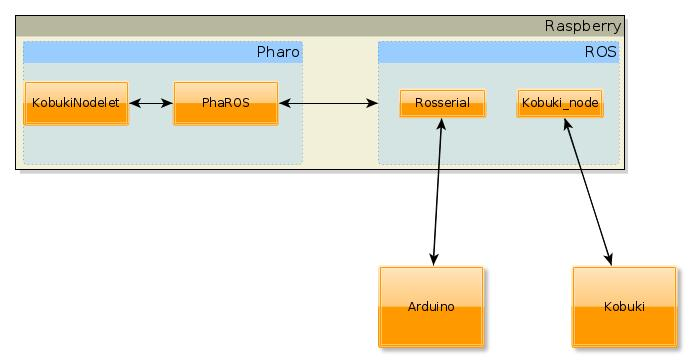
\includegraphics[width=\linewidth]{./architecture.jpg}
  \caption{Architecture générale}
  \label{archi_generale}
\end{center}
\subsection{Arduino}
Le code pour l'Arduino se trouve a l'url
:\\ \url{https://github.com/mattonem/ironminesarduino.git}.

Basiquement, on utilise la librairie fournie par Rosserial pour
pouvoir publier différents topiques sur le port série ainsi que souscrire
à d'autre. On publie les données relatives au contacteur de démarrage
et au capteurs ultrasons. On souscrit aux différents topiques concernant
les actions a effectuer (activer le canon, bouger le bras
rétractable).

\subsubsection{Subscribed Topics}

\begin{itemize}
\item \texttt{/canonTrigger (std\_msgs/Bool)}\\ 
  Si msg.data == true :
  déclenche l'électrovanne pour faire tirer le canon.
\end{itemize}

\subsubsection{Published Topics}

\begin{itemize}
\item \texttt{/sonar/<i> (std\_msgs/UInt16)}\\
  Donne la distance au mur en face du sonar \texttt{i}.\\
  Aujourd'hui, \texttt{i} est compris entre 0 et 4
\item \texttt{/startTrigger (std\_msgs/Bool)}\\ 
  Donne les fronts montant et descendant pour le cordon de démarrage.
\end{itemize}

\subsection{PhaROS - Ironmines}

\begin{center}
  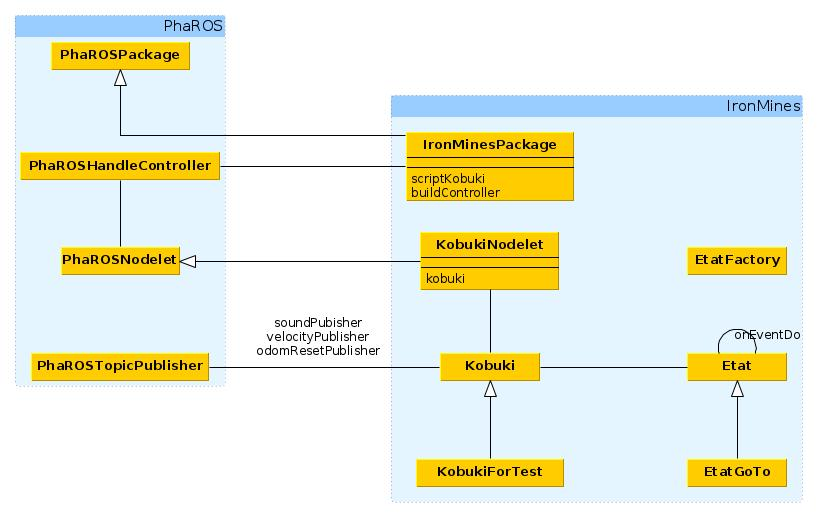
\includegraphics[width=\linewidth]{./UMLClass.jpg}
  \caption{Diagramme de classe}
  \label{dia_class}
\end{center}

Le point d'entrée dans le programme est \texttt{IronMinesPackage} et
sa méthode \texttt{scriptKobuki}. C'est cette méthode qui va lancer
l'instantiation de l'ensemble des entités nécessaires pour le
programme. Va suivre l'instantiation du \texttt{Controller} et son
association avec les nodelets utilisées (ici on utilise uniquement
\texttt{PhaROSTransformationNodelet} et
\texttt{KobukiNodelet}). \texttt{KobukiNodelet} s'occupe alors de la
création d'un objet \texttt{Kobuki}, qui est une représentation
logique du robot.

On peut alors affecter au Kobuki des états. Ceux-ci représentent les
actions qu'on lui demandera de faire (ex: \texttt{EtatGoTo}). Un état
hérite de la classe \texttt{Etat}, et peut définir dans la méthode
\texttt{action} la (les) action(s) actions à effectuer. À la fin de
l'action, si l'état doit finir et mener sur un autre état (ce n'est
pas le cas de tous), on pourra alors appeler la méthode
\texttt{onFinish}. 

Il existe différentes façon de sortir d'un état. La première est
déclenché lorsque l'état est terminé (\texttt{onFinish}). Les autres
peuvent être personnalisées : \texttt{onObstacle},
\texttt{onBumperEvent}. Chacune de ces portes de sorties sont
paramétrées à l'instantiation par la factory. Exemple :

\begin{code}
  newEtat := EtatFactory createGoTo: (0 @ 1) onObstable: unEtatdEvitement next: etatSuivant.
  kobuki changeEtat: newEtat.
  "NB : je ne présente pas ici une interface finalisee, ces methodes sont susceptibles de changer"
\end{code}

Ici on crée un nouvel état qui demandera de kobuki de se rendre en
\texttt{(0,1)}, puis de passer à l'état \texttt{etatSuivant}, mais en
cas d'obstacle on passera a l'état \texttt{unEtatdEvitement}.  Comme
on peut le voir dans le graphique d'objet suivant (représentant le
kobuki au départ d'un script pour tirer sur le mammouth) les états
peuvent former des graphes complexes.
\begin{center}
  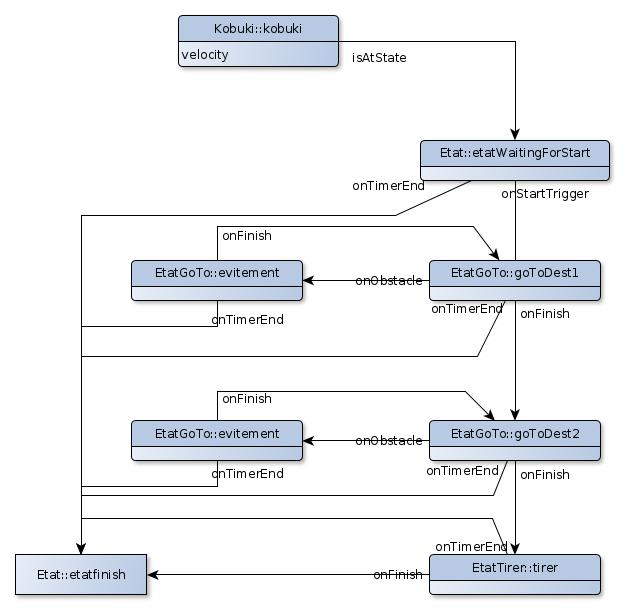
\includegraphics[width=\linewidth]{./UMLObjectEtat.jpg}
  \caption{Diagramme d'objets}
  \label{dia_obj}
\end{center}

\end{document}
